\documentclass{beamer}

\usetheme{Madrid}

\usepackage[orientation=portrait,size=a1,scale=1]{beamerposter}
\usepackage[overlay]{textpos}

\usepackage[utf8]{inputenc}
\usepackage{default}
\usepackage{changepage}
\usepackage{subfigure}
\usepackage{graphicx}
\usepackage[labelformat=empty]{caption}

\setlength{\columnsep}{5cm}
\setlength\labelsep{\dimexpr\labelsep + 0.6em\relax}  

\newlength{\wideitemsep}
\setlength{\wideitemsep}{\itemsep}
\addtolength{\wideitemsep}{10pt}
\let\olditem\item
\renewcommand{\item}{\setlength{\itemsep}{\wideitemsep}\olditem}

\usepackage{tikz}
\usetikzlibrary{calc}
\tikzset{egrid/.style={draw,help lines}}
\tikzset{mgrid/.style={draw,help lines,dashed}}
\tikzset{epoint/.style={draw,circle,red,inner sep=2pt,fill}}
\tikzset{mpoint/.style={draw,circle,blue,inner sep=2pt,fill}}

\definecolor{dark}{RGB}{0,105,0}

\setbeamertemplate{background canvas}[vertical shading][top=yellow!80!dark,bottom=yellow!60!dark]
\beamertemplatenavigationsymbolsempty
\setbeamertemplate{blocks}[rounded][shadow=false]
\setbeamercolor{block body}{bg=yellow!30}
\setbeamercolor{block title}{bg=dark}
\setbeamercolor{item}{fg=dark}
\setbeamertemplate{footline}[page number]{}

\title{Modelling light propagation through \\ radial-director liquid crystal waveguides}

\author{\underline{Miha \v Can\v cula\inst{1}}\and Miha Ravnik\inst{1,2}\and Slobodan \v Zumer\inst{1,2,3}}
\institute{\inst{1}Faculty of Mathematics and Physics, University of Ljubljana, Slovenia\and\inst{2}Centre of excellence NAMASTE, Ljubljana, Slovenia\and\inst{3}Jo\v zef Stefan Institute, Ljubljana, Slovenia}

\newcommand{\blockpadding}{
  \rule[-0.6ex]{0pt}{2.5ex}
}

\addtobeamertemplate{block begin}
  {\vspace{1ex}}
  {\vspace{1ex} % Pads top of block
     % separates paragraphs in a block
   \setlength{\parskip}{24pt plus 1pt minus 1pt}%
   \begin{adjustwidth}{5mm}{5mm}
}
\addtobeamertemplate{block end}
  {\end{adjustwidth}%
   \vspace{1ex}}% Pads bottom of block
  {} % Seperates blocks from each other

\begin{document}

\begin{columns}
 \begin{column}{.976\textwidth}
  \begin{block}{}
\vspace{0.5cm}
\centering
{\fontsize{80}{96}\selectfont \inserttitle} \\
\vspace{1cm}
{\LARGE \underline{Miha \v Can\v cula$^{1}$}, Miha Ravnik$^{1,2}$, Slobodan \v Zumer$^{1,2,3}$} \\
\vspace{1cm}
{\large
$^{1}$Faculty of Mathematics and Physics, University of Ljubljana, Slovenia\\
$^{2}$Centre of excellence NAMASTE, Ljubljana, Slovenia \\
$^{3}$Jo\v zef Stefan Institute, Ljubljana, Slovenia
}
\vspace{0.5cm}
\end{block}


 \end{column}
\end{columns}
\begin{columns}[t]
 \begin{column}{.36\textwidth}
\begin{block}{\blockpadding Motivation}
\begin{itemize}
 \item Light guiding is central in complex optics and photonics, for example for efficient data transfer
 \item Combined birefringence and response to external stimuli in liquid crystal structures could be used for directed guiding of light -- such as waveguides.
 \item Smectic A fibres with radial director profile can be created using 8CB and a surfactant\cite{musevic-nekej}
 \item Point defect in a nematic droplet turns a Gaussian beam into Laguerre-Gaussian -- is there a similar effect caused by the line defect in a fibre?
\end{itemize}
\end{block}

\begin{block}{\blockpadding Methods}
 \begin{itemize}
  \item FDTD method -- direct time evolution of electromagnetic fields in 3D with fully anisotropic $\varepsilon$
  \item Assumed zero conductivity and vacuum permeability in bulk. 
  \item Simulate long cylindrical waveguide with periodic boundary conditions in $z$ direction
  \item Staggered grid, adapted for dielectric anisotropy
  \begin{figure}[h]
\centering
 \subfigure{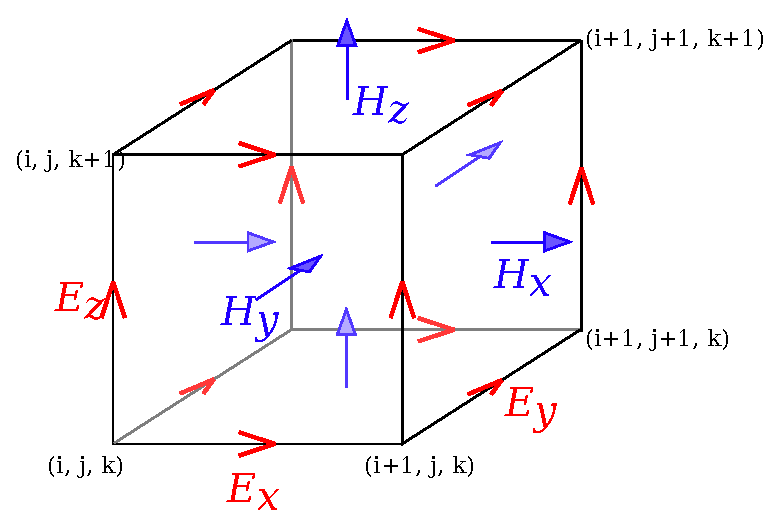
\includegraphics[width=.4\textwidth]{../Magisterij/Slike/Yee-cube}}
 \subfigure{\begin{tikzpicture}[scale=1.4]
    
    \foreach \x in {0,1}{
      \foreach \y in {0,1}{
        \node[mpoint] at (2*\x,2*\y) {}; 
        \node[mpoint] at (2*\x+1.2,2*\y+0.8) {}; 
        \node[epoint] at (2*\x+1.6,2*\y+1.4) {};
        \node[epoint] at (2*\x+1.6-1.2,2*\y+1.4-0.8) {};
        \draw[mgrid] (2*\x,2*\y) -- (2*\x+1.2,2*\y+0.8);
        \draw[egrid] (2*\x+1.6,2*\y+1.4) -- (2*\x+1.6-1.2,2*\y+1.4-0.8);
      }
    }
    
    \draw[mgrid] (0,0) rectangle (2,2);
    \draw[mgrid] (1.2,0.8) rectangle (3.2,2.8);
    \draw[egrid] (1.6,1.4) rectangle (3.6,3.4);
    \draw[egrid] (1.6-1.2,1.4-0.8) rectangle (3.6-1.2,3.4-0.8);
\end{tikzpicture}}
\label{fig:lattice}
\caption{{\color{dark} Left:} Yee lattice, optimized for diagonal dielectric tensor. \\{\color{dark} Right:} The lattice we used, suitable for full anisotropic $\varepsilon$. \\In both cases $\vec E$ and $\vec H$ are known at different times}
\end{figure}
  \item Tested with uniform director, refraction on interfaces, and periodic modulation of refraction index
  \end{itemize}
  \end{block}
  
  \begin{block}{\blockpadding Parameters}
  \begin{itemize}
  \item Observe propagation of Gaussian laser pulse

\item Cylindrical waveguide with a radial director profile and a singular disclination line along its axis [TODO: Prerez] \\
\begin{figure}[h]
\centering
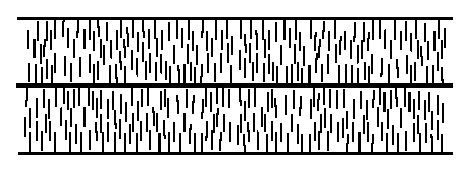
\includegraphics[width=.5\textwidth]{../Magisterij/Slike/director-profile-radial}
\end{figure}
The core radius of the central +1 disclination line is much smaller than the wavelength and can therefore be neglected. 
\item Waveguide radius 10$\mu$m, inside 8CB with $n_o = 1.52$ and $n_e = 1.67$, surrounded by water with $n = 1.33$
\item Mesh size $256 \times 256 \times 128$.

 \end{itemize}
 \end{block}
 
 \begin{block}{\blockpadding References}
  
 \end{block}


 \end{column}
 
 \begin{column}{0.596\textwidth}
  \begin{block}{\blockpadding Electric field}
  \begin{itemize}
   \item We showed that a Gaussian beam entering a fibre quickly turns into a Laguerre-Gaussian beam, and then [into something else]. 
\begin{figure}[h]
\centering
 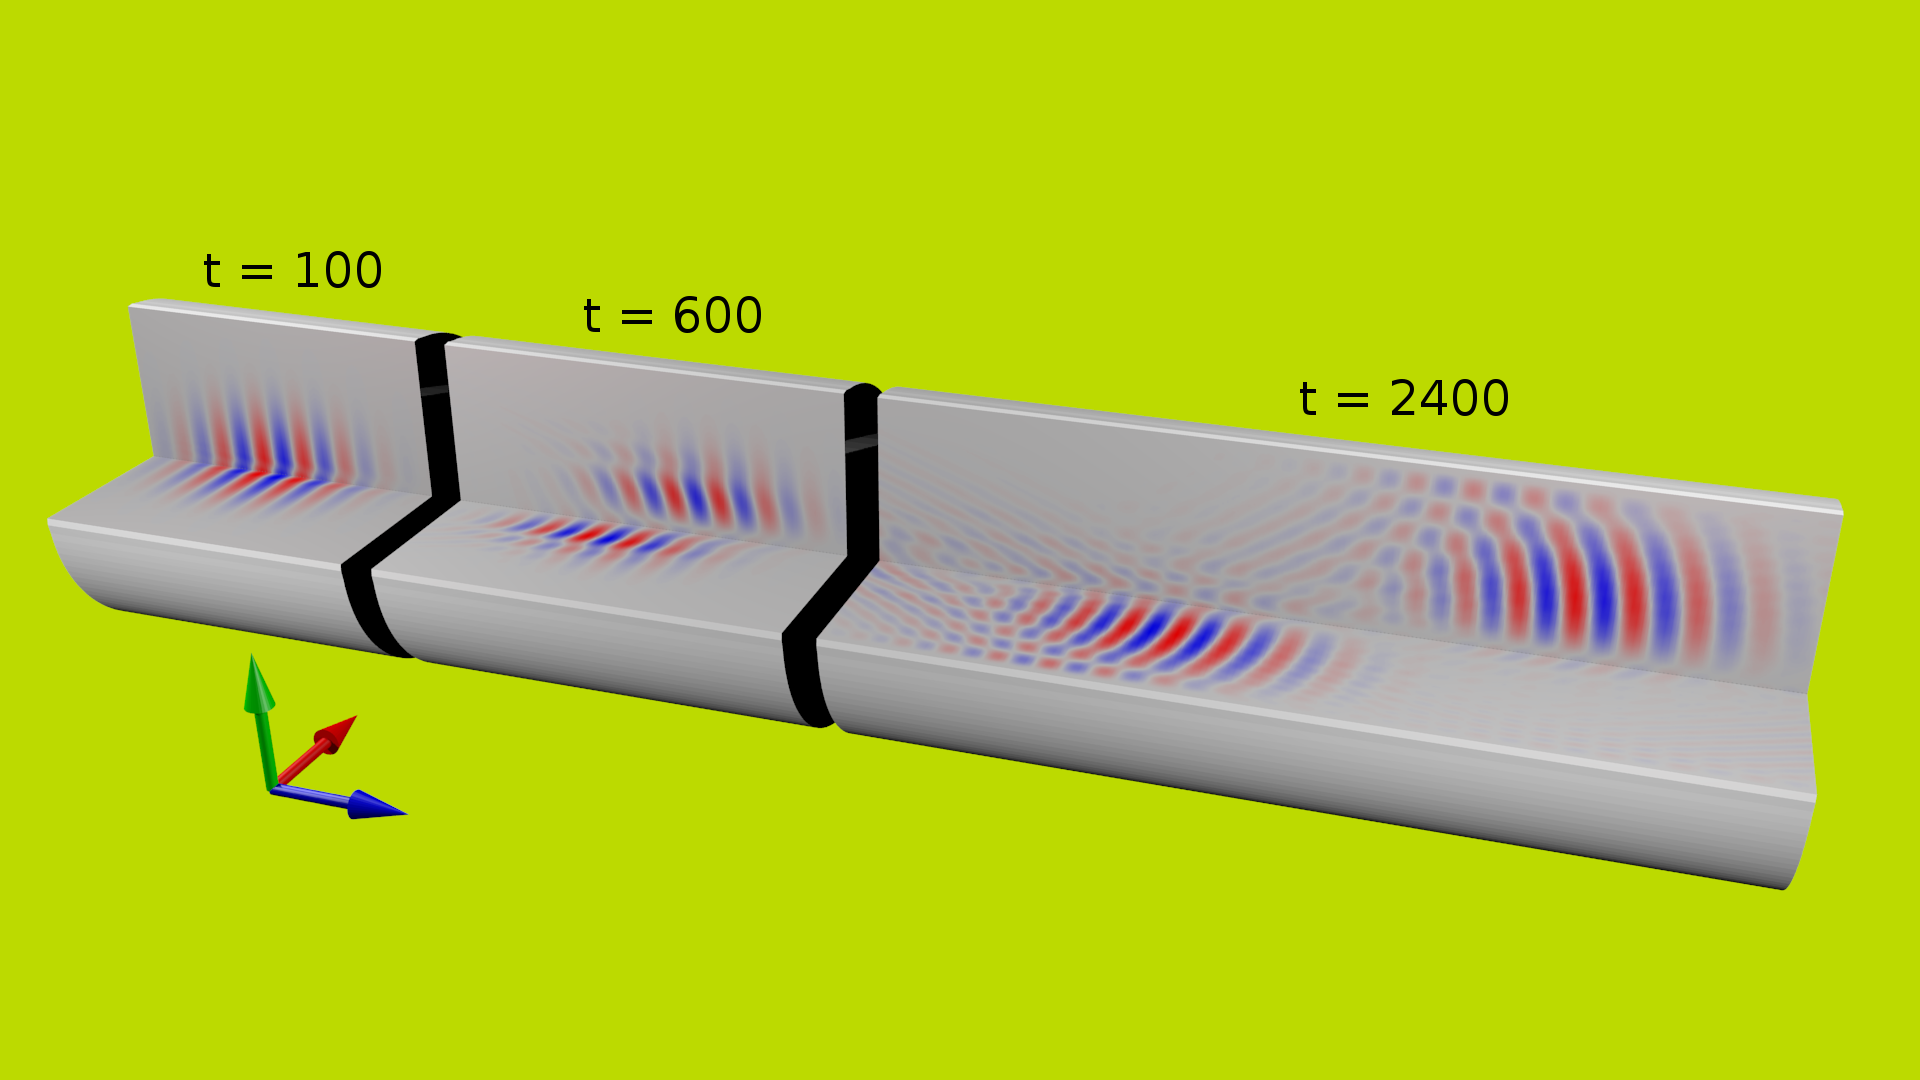
\includegraphics[width=.825\textwidth,clip,trim=0mm 50mm 0mm 80mm]{./render_t}
 \caption{Snapshots of electric field $\vec E$ at three different times. Incident light is polarized along the $x$ axis. {\color{dark} Left:} The Gaussian pulse just after entering the waveguide. {\color{dark} Center:} After a short time, a dark spot forms near the axis. Light near the $xz$ and $yz$ plane differs both in phase and propagation velocity. {\color{dark} Right:} After a longer time, the difference in velocity greatly distorts the pulse. Reflection from waveguide walls causes noticeable interferrence and waveforms lose clarity, although the pattern remains visible. }
\end{figure}
\end{itemize}

\end{block}
\begin{block}{\blockpadding Field intensity and phase}
\begin{itemize}
 \item Using data for electric and magnetic fields we calculated the local energy density. This enabled us to determine the shape of the pulse in time. 
 \begin{figure}[h]
  \centering
  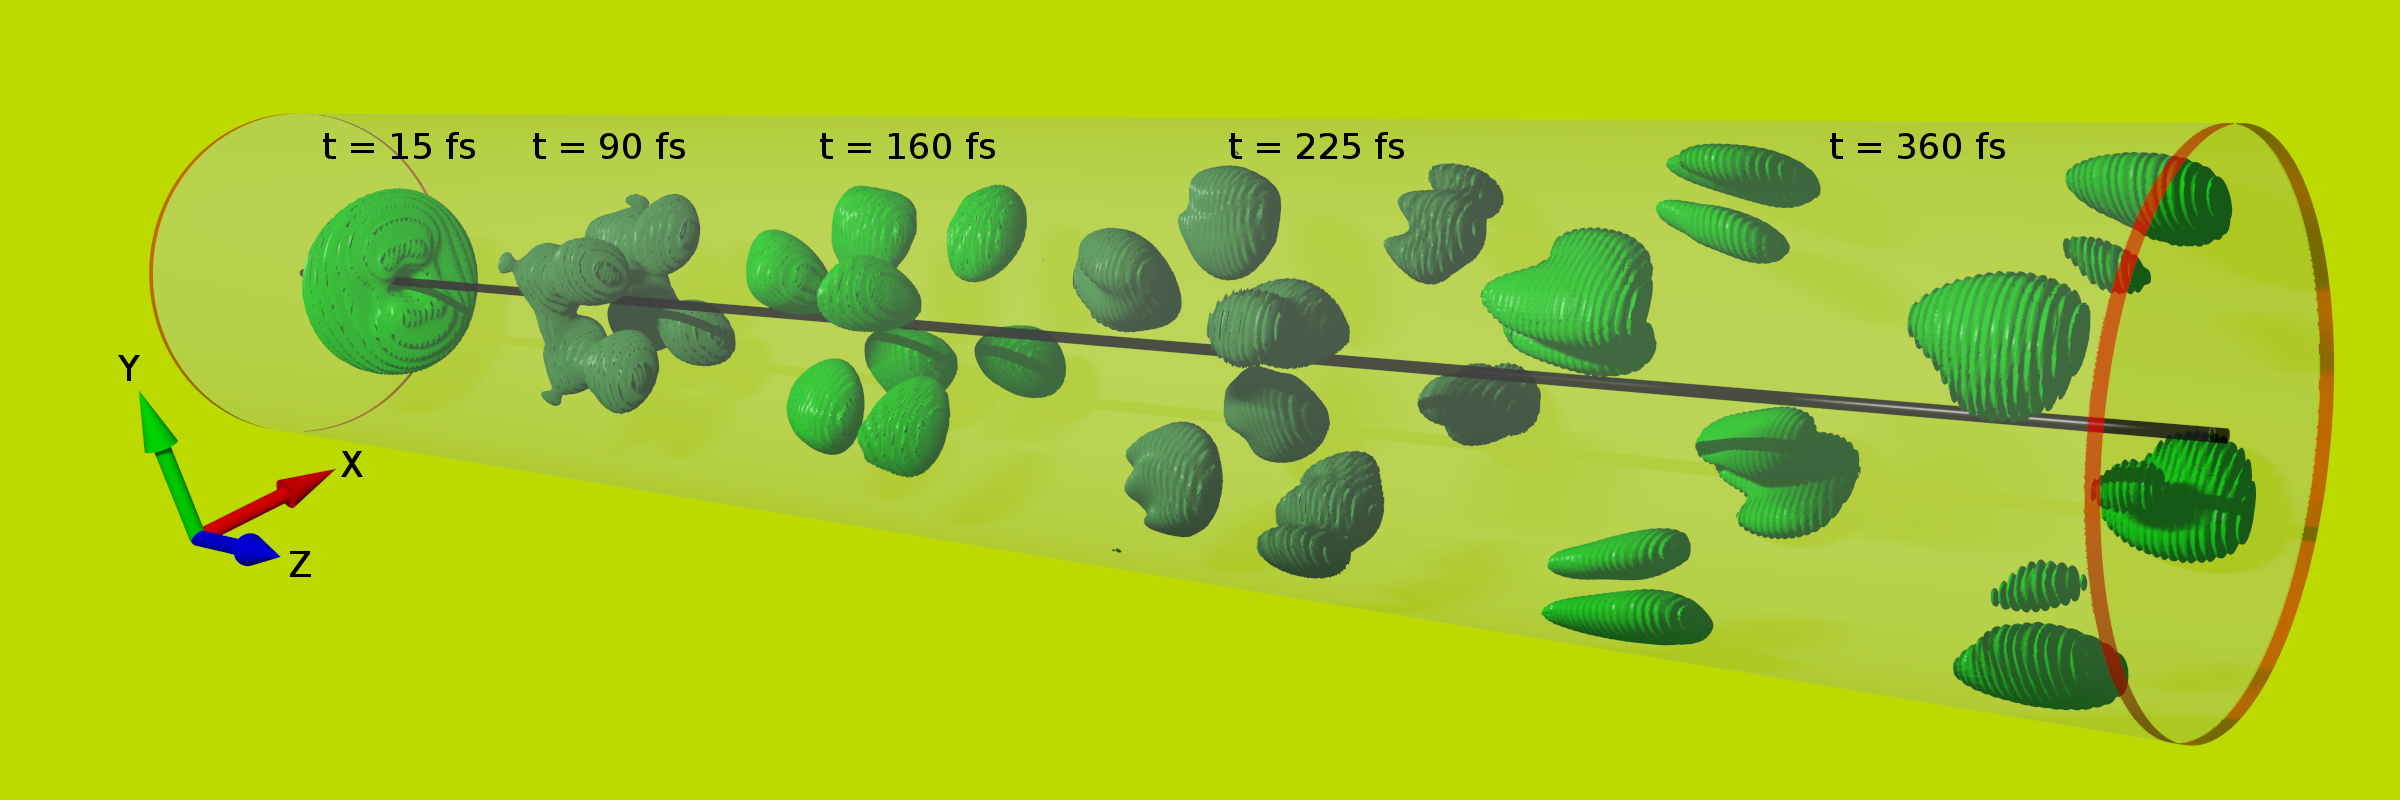
\includegraphics[width=.825\textwidth]{./intensity_gauss_t}
  \caption{Shape of the originally Gaussian pulse at different times after entering the waveguide. Plotted are the isosurfaces where local field amplitude is greater than 5\% of the maximum. At first, the pulse is roughly spherical. Soon a minimum forms at the axis, and the upper and lower parts start overtaking the left and right ones, due to the difference in refraction indexes. The pulse gradually splits into 8 parts, which appears to be a stable configuration. }
 \end{figure}
 \item The pulse splits into multiple intensity regions. Note that the regions are positioned diagonally to the incident light polarization. 

 \item We were also interested in planes of constant phase. By calculating the wave phase at every grid point, we determined that the initially Gaussian pulse quickly transforms into [\v se vedno ne vem kaj]. 
\end{itemize}


\end{block}

\begin{block}{\blockpadding Conclusions}
 \begin{itemize}
  \item A method was developed to model the propagation of light through structures with non-uniform anisotropic dielectric tensor
  \item The method was tested to produce correct results for reflaction and reflection of light, as well as for the photonic band-gap in periodic structures
  \item When applied to a radial-profile liquid crystal waveguide, the method predicts the splitting of a single pulse into eight intensity regions, aligned diagonally around the axis in two ranks
 \end{itemize}

\end{block}

 \end{column}

\end{columns}

\begin{textblock}{5.5}(0.5,5.75)
 

\end{textblock}

\begin{textblock}{8.5}(6.5,2.5)

\end{textblock}

\end{document}
